\myslide{Parser-Autovervollständigung}
{
  \begin{itemgroup}{Übersicht}
    \item Die Parser waren sehr unübersichtlich strukturiert
    \item Pro Ausdruck und Typ wurde ein eigenes \glqq non terminal\grqq eingeführt
    \item Zusätzlich ein eigenes \glqq error non terminal\grqq, welches sich um
          die eingeführte Fehlerbehandlung kümmert
    \item Jedem geparsten Ausdruck wird seine Source Code Position mitgegeben, um
          Fehler anzeigen zu können und, um den Source Code durch die Outline
          markieren zu lassen
    \item Eine automatische Vervollständigung wurde eingeführt, um vom Benutzer
          eingegebene, noch unvollständige Ausdrücke zu vervollständigen
    \item Fehlermeldungen, die mehrere Stellen betreffen, wurden eingeführt
  \end{itemgroup}
}

\myslide{Parser-Autovervollständigung}
{
  {\bf Fehlermeldungen}\\[2mm]
  Gibt der Anwender \glqq \ExprInfixOperation{+}{1}{\KeyLet\ \ExprIdentifier{x} =}\grqq\ 
  ein, wird der Teil \glqq \KeyLet\ \ExprIdentifier{x} =\grqq\ hervorgehoben und der Tooltip
  verrät dem Anwender, dass er noch den Ausdruck \glqq $e_1$\ \KeyIn\ $e_2$\grqq\ eingeben muss,
  um \glqq{\bf Let}\grqq\ zu vervollständigen.
  \begin{center}
    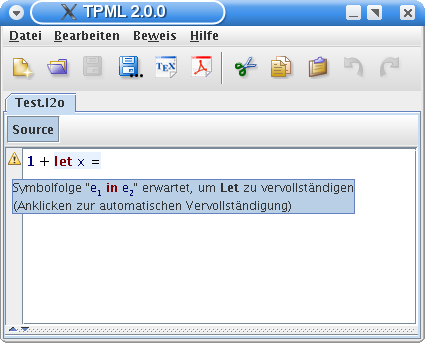
\includegraphics[height=9cm]{images/parser.png}
  \end{center}
}